%%%%%%%%%%%%%%%%%%%%%%% file template.tex %%%%%%%%%%%%%%%%%%%%%%%%%
%
% This is a general template file for the LaTeX package SVJour3
% for Springer journals.          Springer Heidelberg 2010/09/16
%
% Copy it to a new file with a new name and use it as the basis
% for your article. Delete % signs as needed.
%
% This template includes a few options for different layouts and
% content for various journals. Please consult a previous issue of
% your journal as needed.
%
%%%%%%%%%%%%%%%%%%%%%%%%%%%%%%%%%%%%%%%%%%%%%%%%%%%%%%%%%%%%%%%%%%%
%
% First comes an example EPS file -- just ignore it and
% proceed on the \documentclass line
% your LaTeX will extract the file if required
\begin{filecontents*}{example.eps}
%!PS-Adobe-3.0 EPSF-3.0
%%BoundingBox: 19 19 221 221
%%CreationDate: Mon Sep 29 1997
%%Creator: programmed by hand (JK)
%%EndComments
gsave
newpath
  20 20 moveto
  20 220 lineto
  220 220 lineto
  220 20 lineto
closepath
2 setlinewidth
gsave
  .4 setgray fill
grestore
stroke
grestore
\end{filecontents*}
%
\RequirePackage{fix-cm}
%
%\documentclass{svjour3}                     % onecolumn (standard format)
%\documentclass[smallcondensed]{svjour3}     % onecolumn (ditto)
\documentclass[smallextended]{svjour3}       % onecolumn (second format)
%\documentclass[twocolumn]{svjour3}          % twocolumn
%
\smartqed  % flush right qed marks, e.g. at end of proof
%
\usepackage{amsmath}
\usepackage{bm}
\usepackage{graphicx} % Allows including images
\usepackage{epstopdf}
\usepackage{algorithm}
\usepackage[noend]{algpseudocode}
\usepackage[round]{natbib}
\usepackage{amsfonts} % for mathbb
\usepackage{tikz}
% \usepackage[capitalize]{cleveref}
\usetikzlibrary{bayesnet}
\setcitestyle{aysep={ }} %Author-Year Separator
%
% \usepackage{mathptmx}      % use Times fonts if available on your TeX system
%
% insert here the call for the packages your document requires
%\usepackage{latexsym}
% etc.
%
% please place your own definitions here and don't use \def but
% \newcommand{}{}
%
% Insert the name of "your journal" with
% \journalname{myjournal}
%

%%%%%%%%%%%%%%%%%%%%%%%%%%%%%%%%%%%%%%%%%%%%%%%%%%%%%%%%%
% CUSTOM COMMANDS

\newcommand{\bigo}{\mathcal{O}} % NOTE(tim): if you prefer normal O change it here.

\newcommand{\paren}[1]{\mathopen{}\mathclose\bgroup\left(#1\aftergroup\egroup\right)}
\newcommand{\brock}[1]{\mathopen{}\mathclose\bgroup\left[#1\aftergroup\egroup\right]}
\newcommand{\curly}[1]{\mathopen{}\mathclose\bgroup\left\{#1\aftergroup\egroup\right\}}
\newcommand{\anglebrackets}[1]{\langle #1 \rangle}
\newcommand{\ceil}[1]{\lceil #1 \rceil}
\newcommand{\floor}[1]{\lfloor #1 \rfloor}

\DeclareMathOperator*{\argmin}{arg\,min}
\DeclareMathOperator*{\argmax}{arg\,max}

\newcommand{\todo}[1]{\textcolor{magenta}{#1}}
\newcommand{\tim}[1]{\textit{\textcolor{blue}{#1}}}

%%%%%%%%%%%%%%%%%%%%%%%%%%%%%%%%%%%%%%%%%%%%%%%%%%%%%%%%%

\begin{document}

\title{Learning Discrete-valued Bayesian Networks from Mixed Data%\thanks{Grants or other notes
%about the article that should go on the front page should be
%placed here. General acknowledgments should be placed at the end of the article.}
}
%\subtitle{Do you have a subtitle?\\ If so, write it here}

%\titlerunning{Short form of title}        % if too long for running head

\author{Yi-Chun Chen           \and
        Tim A. Wheeler         \and
        Mykel J. Kochenderfer
}

%\authorrunning{Short form of author list} % if too long for running head

\institute{F. Author \at
              first address \\
              Tel.: +123-45-678910\\
              Fax: +123-45-678910\\
              \email{fauthor@example.com}           %  \\
%             \emph{Present address:} of F. Author  %  if needed
           \and
           S. Author \at
              second address
}

\date{Received: date / Accepted: date}
% The correct dates will be entered by the editor


\maketitle

\begin{abstract}
\todo{
Insert your abstract here. Include keywords, PACS and mathematical
subject classification numbers as needed.
}
\keywords{Discretization \and Bayesian Network \and Continuous Variable}
% \PACS{PACS code1 \and PACS code2 \and more}
% \subclass{MSC code1 \and MSC code2 \and more}
\end{abstract}

%%%%%%%%%%%%%%%%%%%%%%%%%%%%%%%%%%%%%%%%%%%%%%%%%%%%%%%%%%%%%%%%%%%%%%%%%%%%%%%%%%%%%%

\section{Introduction}
\label{intro}
Bayesian networks \citep{Pearl_1988, PGM_2009} are an increasingly popular method for modeling uncertainty and causality in science and engineering. They provide an efficient factorization of the joint probability distribution over a set of random variables. Bayesian networks first emerged from artificial intelligence research and have been applied to a wide variety of problems, ranging from decision-making systems \citep{DMU_2015} to medical diagnoses~\todo{[cite]}. In most cases, we assume that all random variables in Bayesian networks are discrete, since many Bayesian network learning algorithms are unable to deal with continuous variables efficiently. However, many applications
require the use of continuous variables, such as position and velocity in dynamic systems.

There are two common approaches to extending Bayesian networks to continuous variables. The first is to model the conditional probability density of each continuous variable using specific families of parametric distributions, and then to redesign Bayesian network learning algorithms based on their parameters. One successful example is belief propagation in Gaussian graphical models \citep{Weiss_2011}. For other particle shapes \citep{Ihler_2009} and non-linear functions \tim{cite if you can}, these redesigned algorithms are computationally expensive and do not perform well.
\tim{Not sure what `particle shapes' are. Do you mean other parametric distributions?}

The second approach is discretization. Automated discretization methods have been studied in machine learning and statistics for many years \citep{Dougherty_1995, Kerber_1992, Holte_1993, Fayyad_1993}. Most discretization methods were designed for classification problems. They search for the best discretization policy\tim{maybe `scheme' is a better word than `policy', which in machine learning means something else.} of a continuous attribute by considering its interation with the target class variable. These discretization methods do not apply to continuous variables in Bayesian networks, where interations and dependencies between variables are more complicated. Discretization of a continuous variable in a Bayesian network requires considering the impact on the entire network. There is prior work on discretizing continuous variables in naive Bayesian networks and tree-augmented networks \citep{Fried_naive}, but only a few discretization methods for general Bayesian networks have been proposed \citep{Friedman_1996, Kozlov_1997, Monti_1998, Steck_2007}.

The discretization technique proposed by \citet{Friedman_1996} is the most well-known of these methods. It is based on the minimum description length principle (MDL): the optimal discretization policy minimizes the description length of the Bayesian network and discretization scheme. The MDL algorithm has a $\bigo\paren{N^3 + \paren{n_c {v_\text{max}}^{(n_c^p)_\text{max}} + {v_\text{max}}^{n_p}} \cdot N^2}$ runtime on Bayesian networks with a single continuous variable and multiple discrete variables, where $N$ is the number of data samples from the joint distribution, $n_p$ and $n_c$ are the numbers of parent and children variables for the continuous variable, $v_\text{max}$ is the largest cardinality over all variables in the Markov blanket, and  ${(n_c^p)_\text{max}}$ is the largest number of parent variables of the continuous variable's children. The MDL method iterates over all continuous variables until convergence in the case of multiple continuous variables, converging in a few cycles according to our tests of real-world data. Unfortunately, MDL tends to produce discrete variables with low cardinality.
\tim{Note: use $\text{thing}$ for subscripts such as $n_\text{max}$.}

\tim{Motivate / introduce Bayesian discretization methods perhaps? This would be a good place to cite Boulle and Lustgarten}

\tim{
The commented material below is good, but feels like too much detail for the intro. Is it possible to move it to later sections?
I recommend having one paragraph that starts with `In this paper we propose \ldots' and then lists the specific contributions. (Bayesian discretization for arbitrary networks, a faster algorithm, demonstrate that performance is preserved, etc.). Then we should have the final paragraph below that discusses organization.}

% In this paper, we propose a new Bayesian discretization method for continuous variables in Bayesian networks. This method extends the Bayesian single-variable discretization methods from \citet{Boulle_2006} and \citet{Lustgarten_2011}. We begin our method with the assumption that only one variable in a given Bayesian network is continuous and other variables are discrete. Furthermore we assume that the network structure is known in advance. Under this situation, we look for the most probable discretization policy $M$ given the data $D$ on other discrete variables. That is to say, the desired policy is $\textrm{arg}_M P(M \mid D)$. With Bayes' rule, $P(M \mid D) $ can be rewritten as $P(M) \cdot P(D \mid M) / P(D)$ , which is proportional to $P(M)\cdot P(D \mid M)$. Usually, $P(D \mid M)$ increases as the number of discretized intervals increases, since more intervals can provide more accuracy. $P(M)$, on the other hand, is designed to decrease as the number of intervals rises. As a result, we can automatically determine the number of intervals after discretization by maximizing  $P(M)\cdot P(D \mid M)$. In addition, the $P(D \mid M)$ can be factorized according to Bayesian network structure. With the proposed priors, we are able to restrict the number of discretized intervals so that it will not exceed the largest cardinality of variables in the Markov blanket by too much. This is important, since for most algorithms on Bayesian networks, their running times exponentially depend on the cardinality of variables. Another advantage of our method is the running time for learning. If there is only one continuous variable, the running time is $O(n_c  {v_\text{max}} \cdot N^2 + {v_\text{max}}^{n_p} \cdot N^2)$, which is significantly shorter than the running time of MDL principle discretization \citep{Friedman_1996}. With the approximation proposed in this paper, we can further reduce running time to $O({v_\text{max}}(n_p+n_c)N^2)$.

% For a Bayesian network with multiple continuous variables, we apply the discretization method discussed above iteratively. In the beginning, we prediscretize each continuous variable by equal-width method. The number of intervals for equal-width discretization is equal to largest cardinality of discrete variables. Then we iterate the one-variable discretization on each continuous variable in the following order: from the variable with highest topological order (leaves) to the variable with lowest topological order (root). Each time we finish a discretization procedure on one variable, we store the discretization result for later iterations. Experiments on real-world data show that with the same iteration order, our discretization method provides better discretization results than MDL principle method in terms of likelihood. The MDL principle method is easily stuck at local minima and also discretizes variables into too few intervals.

% Finally, we can combine our new discretization method with the K2 structure learning alorithm \citep{K2}. We first prediscretize all continuous variables before the K2 learning, since the K2 algorithm requires all variables to be discrete. Each time an edge is added in the K2 algorithm procedure, we rediscretize the continuous variables based on the updated Bayesian network and store the result for the next K2 algorithm iteration. By this principle, we are able to learn a discrete-valued Bayesian network from mixed data.

The rest of the paper is organized as follows: related work, including MDL principle discretization \citep{Friedman_1996} and MODL discretization \citet{Boulle_2006} are summarized in Section \ref{sec:related_work}. Preliminaries and notation are covered in Section \ref{sec:preliminaries}. The proposed single-variable discretization method is derived in Section \ref{sec:single_var} and is extended to Bayesian networks with multiple continuous variables and combined with Bayesian structure learning in Section \ref{sec:multi_var}. The paper concludes with the comparison of the proposed methods against prior work on real-world data in Section \ref{sec:experiments}.

%%%%%%%%%%%%%%%%%%%%%%%%%%%%%%%%%%%%%%%%%%%%%%%%%%%%%%%%%%%%%%%%%%%%%%%%%%%%%%%%%%%%%%

\section{Related Work}
\label{sec:related_work}
This section reviews MDL principle discretization \citep{Friedman_1996} and MODL discretization \citep{Boulle_2006}. The former is the predominant discretization method for continuous variables in Bayesian networks, and is compared to our proposed method in Section \ref{sec:experiments}. The latter is a discretization method for one continuous variable against a discrete target class. Our proposed method generalizes the MODL Bayesian discretization approach to Bayesian networks. The asymptotical equivalence between the MDL and MODL methods were examined in \citep{VL_2000}.

\subsection{MDL Principle Discretization}
The MDL principle was first proposed by \cite{MDL_1978}, and states that the best model for a dataset is one which minimizes the amount of information needed to describe it \citep{Grunwald_2009}. MDL methods trade off goodness-of-fit against model complexity to avoid overfitting. In the context of Bayesian networks, \cite{Friedman_1996} applied the MDL principle to determine the optimal number of discretization intervals for continuous variables and optimal the positions of their discretization boundaries. Their approach selects a discretization policy that minimizes the sum of the description length of discretized Bayesian network and the description length of the information necessary for recovering the original continuous values from the discretized data. In the single continuous variable case, the objective function is
\tim{Do you need double vertical bars? If we use single bars it might fit without having to use the small font size.}

\begin{small}
\begin{equation}
\begin{aligned}
\frac{1}{2} \log(N) \left\lbrace  \lVert \Pi_{X_i} \rVert (\lVert X^*_i \rVert - 1) +
 {\sum_{j,X_i \in \Pi_{X_i}}} \lVert \Pi_{X^*_j} \rVert (\lVert X_j \rVert - 1) \right\rbrace + \log(\lVert {X^*_i} \rVert) \\
 + (N_i-1) H \left( {{\|X^*_i\| - 1}\over{N_i -1}}  \right) -N \cdot \left[ I(X^*_i,\Pi_{X_i}) + {\sum_{j,X_i \in \Pi_{X_i}}} I(X_j, \Pi_{X^*_j}) \right],
\end{aligned}
\end{equation}
\end{small}

\noindent
where $I(\boldsymbol{A},\boldsymbol{B}) = \sum_{\boldsymbol{a},\boldsymbol{b}} \hat{P}_D (\boldsymbol{a},\boldsymbol{b}) \log {{\hat{P}_D (\boldsymbol{a},\boldsymbol{b})}\over{\hat{P}_D (\boldsymbol{a}),\hat{P}_D (\boldsymbol{b})}}$ \tim{consider deleting the right half of equation} is the mutual information between two discrete variables $\boldsymbol{A}$ and $\boldsymbol{B}$, $\|\boldsymbol{X}\|$ is the cardinality of discrete variable $\boldsymbol{X}$, $X^*_i$ is the discretized version of continuous variable $X_i$ and $H(p) = -p \log(p) - (1-p) \log(1-p)$. The optimal discretization policy is found with dynamical programming. If there are multiple continuous variables in a Bayesian network, we apply the algorithm to one variable at a time and iterate over all continuous variables. While iterating, only one variable is treated as continuous and other continuous variables are discretized based on an initial discretization scheme or the discretization result from a previous iteration.

The network structure is not always known in advance. Bayesian network structure learning can be extended to distributions including continuous variables by alternating between traditional discrete structure learning and optimal discretization. Starting with some preliminary discretization scheme, one applys a structure learning algorithm to identify the locally optimal graph structure. The discretization scheme is refined based on the learned network. The cycle is continued until convergence.

\subsection{MODL Discretization}
\tim{Does MODL stand for something?}
MODL discretization \citep{Boulle_2006} is a Bayesian method for discretizing a continuous feature according to a class variable. Bayesian methods maximize the probability of the model given the data, $P(\textit{Model} \mid \textit{Data})$. An application of Bayes' rule and constant $P(\textit{Data})$ shows that this is equivalent to maximizing:
\begin{align}
P(\textit{Model}) \cdot P(\textit{Data} \mid \textit{Model})\text{,}
\end{align}

\noindent
where $P(\textit{Model})$ is a prior over models and $P(\textit{Data} \mid \textit{Model})$ is the data likelihood.
The data likelihood usually increases with the number of discretization intervals, as more intervals allow for more detailed representations.
The prior usually decreases as the number of discretization intervals increases to favor simpler models and penalize overfitting.
Thus, maximizing $P(\textit{Model}) \cdot P(\textit{Data} \mid \textit{Model})$ requires a trade-off when determining the number of discretization intervals.

The MODL method uses dynamic programming to find the optimal discretization scheme, and has a $\bigo\paren{N^3 + \|\text{Class}\| \cdot N^2}$ runtime, where $N$ is the of number of data instances. \cite{Lustgarten_2011} suggest several formulations for the prior term $P(\text{Model})$\tim{Did I state this correctly?}. If the prior is chosen to reflect uniform prior probability over discretizations the runtime can be reduced to $\bigo\paren{\|\text{Class}\| \cdot N^2}$.\tim{Is a sacrifice made? It is sub-optimal, right?}

%%%%%%%%%%%%%%%%%%%%%%%%%%%%%%%%%%%%%%%%%%%%%%%%%%%%%%%%%%%%%%%%%%%%%%%%%%%%%%%%%%%%%%

\section{Preliminaries}
\label{sec:preliminaries}
This section provides a brief overview of Bayesian networks, including the factorization of joint probability distributions, sampling from a Bayesian network, and structure learning. These concepts will be used in later sections. The formal definition of a discretization policy for a continuous variable is also given.

\subsection{Bayesian Networks and Structure Learning}

A Bayesian network $B$ is defined by a pair $(G,\Theta)$, where $G = (X,E)$ is a directed acyclic graph whose nodes correspond to a set of random variables $X = \brock{X_1, X_2, \cdots, X_n}$, and whose edges $E$ represent probabilistic dependencies among nodes. The graph structure $G$ encodes the Markov property: each node $X_i$ is independent of its non-descendants given its parents $\Pi{X_i}$ in $G$. The conditional relations are parameterized by the elements of $\Theta$, which take the form $\theta_{x_i \mid \Pi_{x_i}} = P(x_i \mid \Pi_{x_i})$ for each possible value $x_i$ of $X_i$, and $\Pi_{x_i}$ of $\Pi_{X_i}$. The joint distribution over $X$ factors according to the Markov property:
\begin{equation}
P_B (X_1 , \cdots, X_n) = \prod_{i=1}^{n} P_B (X_i \mid \Pi_{X_i}) = \prod_{i=1}^{n} \theta_{x_i \mid \Pi_{x_i}}\text{.}
\end{equation}

Samples can be drawn from the joint distribution represented by a Bayesian network by forward sampling.
Variables are sampled in topological order such that parental instantiations are always known~\citep[see][chap.~22]{algo_2009}.
Furthermore, the parent\rightarrow child sampling order can be reversed if the marginal probability of child variable $P(X_i)$ is known.
By Bayes' rule,

\begin{equation}
P(X_i \mid \Pi_{X_i}) \cdot \prod_{j = 1}^{ Pa( X_i)} P( \{ \Pi_{X_i} \}_j) = P(X_i) \cdot P(\Pi_{X_i} \mid X_i),
\end{equation}

\noindent
where $Pa(X_i)$ is the number of parents of $X_i$ and $\brock{\Pi_{X_i}}_j$ is the $j$th parent of $X_i$.
% One can first sample $X_i$ by $P(X_i)$, then sample all the parent variables simultaneously by $P(\Pi_{X_i} \mid X_i)$. That is to say, $X_i$ becomes the starting point of sampling.

It is often necessary to infer the structure of a Bayesian network from data.
Three common approaches to Bayesian network structure learning are constraint-based structure learning, score-based structure learning, and Bayesian model averaging \citep[see][chap.~18]{PGM_2009}. This work uses the K2 structure learning algorithm \citep{K2}, one of the most successful score-based structure learning methods.
Score-based structure learning methods over discrete variables commonly evaluate candidate structures are scored according to their likelihood, $\prod_i f(X_i, \Pi_{X_i})$, where

\begin{align}
f(X_i, \Pi_{X_i}) = \prod_{j=1}^{\|\Pi_{X_i}\|} {{(\|X_i\|-1)!}\over{(N_{ij} + \|X_i\|-1)!}} \prod_{k=1}^{\|X_i\|} \alpha_{ijk}!\text{.}
\end{align}

\noindent
$\|X_i\|$ is the cardinality of $X_i$, $\|\Pi_{X_i}\|$ is number of possible instantiations of the parent variables of $X_i$, $\alpha_{ijk}$ is the number of instances of the $k$th value of $X_i$ and the $j$th parental instantiation, and $N_{ij} = \sum_{k=1}^{|X_i|} \alpha_{ijk}$.\tim{Mykel uses $\alpha_{ij0}$}
The optimal structure is the most probably structure given the data.
The space of acyclic graphcs is superexponential in the number of nodes \citep{PGM_2009} so it is common to rely on heuristic search strategies.

The K2 algorithm assumes a topological ordering of variables and greedily adds parents to nodes to maximally increase the likelihood score.
A fixed ordering ensures acyclicity but does not guarantee a globally optimal network structure.
K2 is typically run multiple times with random topological orderings and the network with the highest likelihood is retained.

\subsection{Discretization Policies}

A discretization policy $M_C = \anglebrackets{t_1 < t_2 < \ldots < t_{k-1}}$ for a continuous variable $C$ is a mapping from $\mathbb{R}$ to $\brock{1,2,3,\ldots,k}$ such that
\begin{equation}
  M_C (x)=\begin{cases}
    1, & \text{if $x<t_1$}.\\
    i, & \text{if $t_{i-1} \leq x < t_i$}\text{.}\\
    k, & \text{if $t_{k-1} \leq x$}
  \end{cases}
\end{equation}

\noindent
The policy discretizes the continuous variable $C$ into $k$ intervals. Furthermore, we restrict the discretization edges $t_\cdot$ to midpoints between two sorted instances of $C$. An integer representation of $M_C$ can be obtained by sorting the samples of $C$ in an increasing order, $\curly{c_1,c_2,\ldots,c_N}$, and if $t_i = (c_{s_{i}} + c_{s_{i}+1})/2$ for $i=1,2,\ldots,k$, then $M_C = \anglebrackets{t_1,t_2, \ldots, t_{k-1}} \equiv \brock{n_1,n_2,..n_k}$, where $n_1 = s_1$ and $n_i = s_{i} - s_{i-1}$ for all $i = 2,\ldots,k$.

%%%%%%%%%%%%%%%%%%%%%%%%%%%%%%%%%%%%%%%%%%%%%%%%%%%%%%%%%%%%%%%%%%%%%%%%%%%%%%%%%%%%%%

\section{Discretization of a Single Continuous Variable}
\label{sec:single_var}

This section covers discretization of a single continuous variable in a Bayesian network where all other variables are discrete.
Before we formulate the objective function, we introduce some notations that will make the following calculation easier.

\subsection{Notations}

\tim{We should move the notation section to preliminaries}

\tim{Earlier the continuous variable was denoted $C$. Now it is $X$. Slightly confusing with $c$ also meaning child.}

Consider continuous variable $X$.
It has $n_p$ parents, $\Pi_X = \{ P_1, P_2, P_3,\ldots,P_{n_p}\}$ and $n_c$ children, $\{ C_1, C_2,\ldots,C_{n_c}\}$.
Each child $C_i$ of $X$ may possess other parents, our spouses of $X$, whose set is denoted $\boldsymbol{S_i}$.

Let $D$ be a dataset of $N$ joint instances from which discretization will be learned, sorted in ascending order according to $X$.
Let $D_{\boldsymbol{Y}}$ will refer to the data instances associated with variables $\boldsymbol{Y}$.
Thus $D_X = \{ x_1,x_2,x_3,\ldots,x_N \}$.
In order to facilitate understanding, we temporarily assume all values in $D_X$ are unique, that is, $x_1 < x_2 < \ldots < x_N$.
It follows that a discretization policy $M$ on $X$ can be written as $M_X = \brock{n_1,n_2,\ldots,n_k}$, where $k$, $n_1$, $n_2$, $\ldots,n_k$ are positive integers satisfying $N = \sum_{i=1}^k n_i$.
The optimal discretization policy maximizes $P(M)\cdot P(D\mid M)$.

%Furthermore, since there might have repeated values for $D_x$, we assume there are $N'$ unique values of $D_x$ and $N' \leq N$. Note that the allowable discretization edges happens between two consective values of non-repeated value of $D_x$. For example, if $D_X = \{ 1.0,1.0,2.0\}$, then the only possible discretization edge is on $1.5$.


\subsection{Priors and Objective Function}

Four prior principles adapted from the MODL approach define $P(M)$ and $P(D \mid M)$:
\begin{enumerate}
\item A discretization edge at $(x_i + x_{i+1})/2$ has probability
\begin{equation}
1 - {\exp(- L \cdot {{x_{i+1} - x_i}\over{x_N - x_1}})},
\end{equation}
where $L$ is the largest cardinality of discrete variables in $X$'s Markov blanket.
\item For a given interval of $M$, every distribution of $\Pi_X$ is equiprobable.
\item For each pair $(C_i,\boldsymbol{S_i})$ and a given interval of $M$, every distribution over $C_i$ given $\boldsymbol{S_i}$ is equiprobable.
\item The distributions over each $C_i$ and $\Pi_X$ in each interval of $M$ given each instantiation of $\boldsymbol{S_i}$ are independent.
\end{enumerate}

The prior term $P(M)$ has the form:

\begin{equation}
\label{eq:p_M}
P(M) = \prod_{i=1}^k \brock{ [1 - {\exp(- L \cdot {{x_{s_i+1} - x_{s_i}}\over{x_N - x_1}})}] \cdot \exp(L \cdot {{x_{s_{i}} - x_{s_{i-1} + 1}}\over{x_N - x_1}}) }\text{,}
\end{equation}

\noindent
where $s_i = \sum_{j=1}^k n_j$, $s_k = N$, and $s_0 = 0$. Before evaluating $P(D \mid M)$, note that

\begin{equation}
\label{eq:p_D_given_M}
P(D \mid M) \propto P(D_{\Pi_x} \mid M) \cdot \prod_{i = 1}^{n_c} P(D_{C_i} \mid M, D_{\boldsymbol{S_i}})\text{.}
\end{equation}

The graph structure allows us to only consider the interations between $X$ and the other variables in its Markov blanket, thus allowing for convenient factorization. For example, $P(D \mid M)$ for Figure \ref{fig:one} factors according to
\begin{equation}
P(D_{ P_1,P_2,P_3 } \mid M) \cdot P( D_{ C_1 } \mid M,D_{\boldsymbol{S_1}}) \cdot P(D_{C_2} \mid M,D_{ S_2  })\text{.}
\end{equation}

\begin{figure}[ht]
    \begin{tabular}{cc}
      % model_pca.tex
%
% Copyright (C) 2012 Jaakko Luttinen
%
% This file may be distributed and/or modified
%
% 1. under the LaTeX Project Public License and/or
% 2. under the GNU General Public License.
%
% See the files LICENSE_LPPL and LICENSE_GPL for more details.

% PCA model

%\beginpgfgraphicnamed{model-pca}
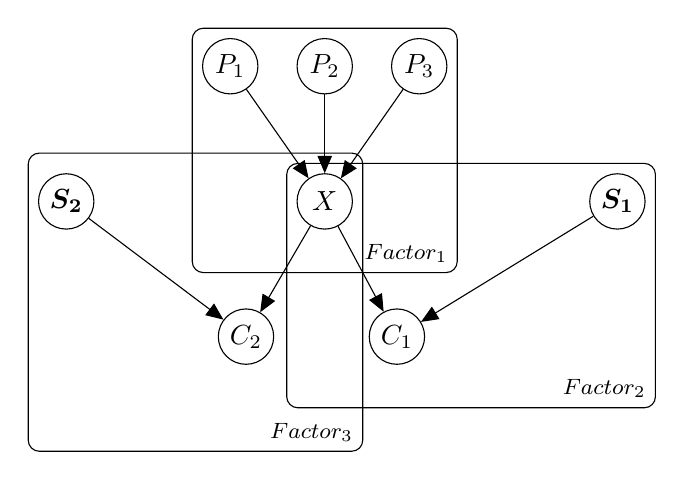
\begin{tikzpicture}

  % Define nodes
  \node[latent]                               (c1) {$C_2$};
  \node[latent, right= 1.2 cm of c1]            (c2) {$C_1$};
  \node[latent, above=of c1, xshift= 1 cm] (y)  {$X$};
  \node[latent, above=of y, xshift=-1.2cm] (p1) {$P_1$};
  \node[latent, above=of y, xshift=0cm]  (p2) {$P_2$};
  \node[latent, above=of y, xshift=1.2cm]  (p3) {$P_3$};
  \node[latent, right= 3.0cm of y]            (s1) {$\boldsymbol{S_1}$};
  \node[latent, right=-4.0cm of y]            (s2) {$\boldsymbol{S_2}$};

  % Connect the nodes
  \edge {p1,p2,p3} {y} ; %
  \edge {y,s1}{c2} ;
  \edge {y,s2}{c1};

  % Plates
  \plate {} {(p1)(p2)(p3)(y)} {$Factor_1$} ;
  \plate {yx} {(y)(s1)(c2)} {$Factor_2$};
  \plate {} {(y)(s2)(c1)(yx.north west)(yx.south west)} {$Factor_3$} ;
  %\plate {} {(w)(y)(yx.north west)(yx.south west)} {$M$} ;

\end{tikzpicture}
%\endpgfgraphicnamed

%%% Local Variables: 
%%% mode: tex-pdf
%%% TeX-master: "example"
%%% End: 

    \end{tabular}
  \caption{Factorization of $P(D \mid M)$}
  \label{fig:one}
\end{figure}

The factorization arises from the conditional independencies in the Bayesian network.
Given a distribution over $X$ and a specific instance $x$, one can directly determine the conditional distribution over the parents $\Pi_x$.
The parents given $x$ are dependent, in general one cannot further factorize $P(D_{\Pi_x} \mid M)$.
Similarly, a distribution over $C_i$ is fully defined given $x$ and $\boldsymbol{S_i}$.
The children are independent given $X$, and thus factorize according to $\prod_{i = 1}^{n_c} P(D_{C_i} \mid M, D_{\boldsymbol{S_i}})$.

It is thus necessary to formulate $P(D_{\Pi_x} \mid M)$  and $P(D_{C_i} \mid M, D_{\boldsymbol{S_i}})$ based on discretization policy $M = [n_1,n_2,\ldots,n_k]$ in order to compute the likelihood term, $P(D \mid M)$. These components are outlined below.

\subsubsection{Evaluation of $P(D_{\Pi_x} \mid M)$}

Let $J_P = \prod_{i=1}^{n_p} \| P_i \|$. It follows that

\begin{equation}
\label{eq:likelihood_one}
P(D_{\Pi_X} \mid M) = \prod_{i=1}^k  {{1}\over{{n_i + J_P - 1}\choose{J_P -1}}}
{{1}\over{ {{{n}_i}!}\over{ {n^{(p)}_{i,1} !} {n^{(p)}_{i,2} !} \cdots {n^{(p)}_{i,J_P} !}}  }}\text{,}
\end{equation}

\noindent
where $n^{(p)}_{i,j}$ is the number of instances in the $i$th discretized interval with the $j$th value of $\Pi_X$.
Note that $n_i = \sum_{j=1}^{\| \Pi_x \|} n^{(p)}_{i,j}$.
The two factors on the right hand side comes from the second prior: all distributions of values of $\Pi_X$ in a given interval are equiprobable. According to the fourth prior, the distribution in each interval is independent, so the two factors are multiplied together.

\subsubsection{Evaluation of $P(D_{C_i} \mid M, D_{\boldsymbol{S_i}})$}

For each pair $(C_j, \boldsymbol{S_j})$, let $\|C_j \| = J_j$ and $\| \boldsymbol{S_j} \| = L_j = \prod_{v \in \boldsymbol{S_j}} \| v \|$. It follows that

\begin{equation}
\label{eq:likelihood_two}
P(D_{C_j}  \mid M, D_{S_j}) =
\prod_{i=1}^{k} \prod_{l=1}^{L_j} {{1}\over{{n_{i,l} + J_j - 1}\choose{J_j-1}}}
{{1}\over{ {{n_{i,l}}!}\over{ {n^{(j)}_{i,1,l} !} {n^{(j)}_{i,2,l} !} \cdots {n^{(j)}_{i,J_j,l} !}}  }}\text{,}
\end{equation}

\noindent
where $n^{(j)}_{i,m,l}$ is the number of instances in $i$th interval with $m$th value of $C_j$ and $l$th value of $\boldsymbol{S_j}$, $n_{i,l} = \sum_{m=1}^{J_j} n^{(j)}_{i,m,l}$, and $n_i = \sum_{l=1}^{L_j} n_{i,l}$.
The two factors on the right hand side come from the third prior: all distribution of values of $C_j$ in a given interval and with a given value of $S_j$ are equiprobable. According to the forth prior, these distributions are independent from each other, and one thus takes their product. If $S_j = \emptyset$, then Equation \ref{eq:likelihood_two} is equivalent to

\begin{equation}
\label{eq:likelihood_three}
P(D_{C_j}  \mid M) =
\prod_{i=1}^{k}  {{1}\over{{n_{i} + J_j - 1}\choose{J_j-1}}}
{{1}\over{ {{n_{i}}!}\over{ {n^{(j)}_{i,1,\emptyset} !} {n^{(j)}_{i,2,\emptyset} !} \cdots {n^{(j)}_{i,J_j,\emptyset} !}}  }}\text{,}
\end{equation}

\noindent
where $n^{(j)}_{i,m,\emptyset}$ is the number of instances in the $i$th interval with the $m$th value of $C_j$, and $\sum_{m=1}^{J_j} n^{(j)}_{i,m,\emptyset} = n_i$.

The objective function can be formulated given equations \ref{eq:p_M}, \ref{eq:p_D_given_M},\ref{eq:likelihood_one}, and \ref{eq:likelihood_three}.
The log-inverse of $P(M) \cdot P(D|M)$ is minimized for computational convenience:

\begin{equation}
\label{eq:opt_prob}
\begin{aligned}
& \sum_{i=1}^{k-1} - \log(1 - {\exp(- L \cdot {{x_{s_i+1} - x_{s_i}}\over{x_N - x_1}})}) +  \sum_{i=1}^{k} L \cdot {{x_{s_{i}} - x_{s_{i-1} + 1}}\over{x_N - x_1}} +\\
&  \sum_{j=1}^{n_c} \sum_{i=1}^{k}  \sum_{l=1}^{L_j} \left[  \log{{n_{i,l} + J_j - 1}\choose{J_j-1}} + \log \left( { {{n_{i,l}}!}\over{ {n^{(j)}_{i,1,l} !} {n^{(j)}_{i,2,l} !} \cdots {n^{(j)}_{i,J_j,l} !}} } \right) \right] + \\
& \sum_{i=1}^k \left[  \log {{n_{i} + J_P - 1}\choose{J_P-1}} + \log \left( { {{n_i}!}\over{ {n^{(p)}_{i,1} !} {n^{(p)}_{i,2} !} \cdots {n^{(p)}_{i,J_p} !}} } \right) \right]\text{.}
\end{aligned}
\end{equation}

\subsection{Algorithm}

This section describes the procedure used to minimize the objective function.
Note that the objective function is cumulative over intervals, thus, if a partition of $X$ into $k$ intervals with lengths $n_1,n_2,\ldots,n_k$ is an optimal discretization policy, then any subinterval is optimal for the corresponding subproblem.
It follows that dynamic programming can be used to solve the optimization problem exactly.

Every midpoint between two nonequal consecutive values in $D_X$ is a candidate discretization edge.
Let ${D'_X} = \brock{x'_1,x'_2,\ldots,x'_M}$ be the set of unique values of $D_X$ sorted in ascending order, where $M$ is the number unique values in $D_X$.
Recall that $D_X$ is also sorted.
Let $b = \brock{b_0,b_1,b_2,\ldots,b_M}$ be an increasing sequence of integers marking the repeated value intervals in $D_X$ such that $b_0 = 0$ and $x_{b_{i-1} + 1} = x_{b_{i-1} + 2} = \ldots = x_{b_i} = x'_i$.
By this definition, the allowable discretization positions are $d_i = \paren{x_{b_{i}} + x_{{b_i}+1}}/2$ for all $i = 1,2,\ldots,M-1$.

Precomutation can be done to reduce runtime.
Compute $h(u,v)$ for each interval $I_q$ starting from $x_{u}$ to $x_{v}$ for all $(u,v)$ satisfying $u \leq v$:

\begin{small}
\begin{equation}
\begin{aligned}
h(u,v) &=  \log {{n_{q} + J_P - 1}\choose{J_P-1}} + \log \left( { {{n_q}!}\over{ {n^{(p)}_{q,1} !} {n^{(p)}_{q,2} !} \cdots {n^{(p)}_{q,J_p} !}} } \right) \\
& + \sum_{j=1}^{n_c} \sum_{l=1}^{L_j} \left[  \log{{n_{q,l} + J_j - 1}\choose{J_j-1}} + \log \left( { {{n_{q,l}}!}\over{ {n^{(j)}_{q,1,l} !} {n^{(j)}_{q,2,l} !} \cdots {n^{(j)}_{q,J_j,l} !}} } \right) \right]
\end{aligned}
\end{equation}
\end{small}

The evaluation of $h(u,v)$ for all $u \leq v$ is summarized in Algorithm \ref{alg:h} in the appendix.
The calculation has a $O(n_c  {v'_\text{max}} \cdot N^2 + {v'_\text{max}}^{n_p} \cdot N^2)$ runtime, where $n_c$ and $n_p$ are the numbers of child and parent variables respectively, and $v'_\text{max}$ is the largest cardinality of variables that directly connect to $X$.

% \tim{I think we can leave this out if it doesn't affect the algorithm results, and people will always sort in ascending order}
% Due to repeated values in $D_X$, for some pairs $(u,v)$, $h(u,v)$ may depend on the sorting method of $D_X$ and $D$.
% However, this does not influence the optimization result, since these pairs of $u$ and $v$ will not form valid intervals.

Now we are able to solve the optimization problem over Equation \ref{eq:opt_prob}.
The dynamic programming procedure is shown in Algorithm \ref{alg:disc_one}.
It takes two inputs: $D$, the joint samples over all variables sorted in ascending order according to $D_X$, and $G$, the network structure.
The runtime of Algorithm \ref{alg:disc_one} is also $O(n_c  {v'_\text{max}} \cdot N^2 + {v'_\text{max}}^{n_p} \cdot N^2)$, because the runtime of the dynamic programming procedure is less than the runtime for computing $h(u,v)$.
Algorithm \ref{alg:disc_one} is guaranteed to be optimal.
For faster methods with suboptimal results please refer to \citep{Boulle_2006}.

\begin{algorithm}
\caption{Discretization of one continuous variable in a Bayesian network}
\label{alg:disc_one}
\begin{algorithmic}[5]
\Function{Discretize}{$D$, $G$}
\State
\State $N \leftarrow$ the number of instances
\State $N' \leftarrow$ the number of unique values in $D_X$
\State $H \leftarrow$ an $N \times N$ matrix such that $H[u,v] = h(u,v)$ per Algorithm \ref{alg:h} in the appendix
\State $b \leftarrow$ the increasing sequence of $M$ integers as previously defined
\State $L \leftarrow$ the largest cardinality over all discrete variables in the Markov blanket of $X$
\State $S[u] \leftarrow$ the optimal objective value of subproblems with instances from $1$ to $u$
\State $M[u] \leftarrow$ the optimal discretization for subproblems with instances from $1$ to $u$
\State $W[u]  \leftarrow - \log(1 - {\exp(- L \cdot{ {{x_{b(u)+1} - x_{b(u)}}\over{x_N - x_1}})}})$ for $u = 1,2, \ldots,N'-1$ and $L(N') \leftarrow 0$
\State
\For {$v = 1$ to $N'$}
\If {$v = 1$}
\State $S[v] \leftarrow g \left(1,b[v] \right) + L[v]$
\State $M[v] \leftarrow \{ ({x_{b[v]} + x_{b[v]+1}}) / 2\}$
\Else
\State $s \leftarrow \infty$ and $boundary \leftarrow \infty$
\For {$u = 1$ to $v$}
\State $s' \leftarrow S[u] + g \left( b[u]+1,b[v] \right) +  {L \cdot {{x_{b[v]} - x_{b[u] + 1}}\over{x_N - x_1}}} + W[v]$
\If {$s' < s$}
\State $s \leftarrow s'$
\State $boundary \leftarrow ({x_{b[u]} + x_{b[u]+1}}) / 2$
\EndIf
\EndFor
\State $S[v] \leftarrow s$
\State $M[v] \leftarrow M[u] \cup \{ boundary\}$
\EndIf
\EndFor
 \State \Return $M$
\EndFunction
\end{algorithmic}
\end{algorithm}


\subsection{Approximation}

Algorithm \ref{alg:disc_one} has an exponential $\bigo\paren{\paren{v'_\text{max}}^{n_p} \cdot N^2}$ runtime.
This exponential runtime is severely limiting for networks with a large number of discretization edges.
This section introduces an approximation to the objective function that significantly reduces the runtime and still preserves the quality of discretization.
The approximation replaces the dominator of the last factor in Equation \ref{eq:likelihood_one} with

\begin{equation}
{\frac{{n_i}!}{ {n^{(p)}_{i,1} !} {n^{(p)}_{i,2} !} \cdots {n^{(p)}_{i,J_P} !}}} \approx \prod_{r=1}^{n_p} { {{{n}_i}!}\over{ {n^{(p_r)}_{i,1} !} {n^{(p_r)}_{i,2} !} \cdots {n^{(p_r)}_{i,J_{p_r}} !}}}\text{,}
\end{equation}

\noindent
where $J_{p_r} = \| P_r\|$ and ${n^{(p_r)}_{i,j} !}$ is the number of instances in the $i$th interval with the $j$th value of $P_r$.
The approximated objective function is

\begin{equation}
\begin{aligned}
\label{eq:opt_prob_approx}
& \sum_{i=1}^{k-1} - \log(1 - {\exp(- L \cdot {{x_{s_i+1} - x_{s_i}}\over{x_N - x_1}})}) +  \sum_{i=1}^{k} L \cdot {{x_{s_{i}} - x_{s_{i-1} + 1}}\over{x_N - x_1}} +\\
&  \sum_{j=1}^{n_c} \sum_{i=1}^{k}  \sum_{l=1}^{L_j} \left[  \log{{n_{i,l} + J_j - 1}\choose{J_j-1}} + \log \left( { {{n_{i,l}}!}\over{ {n^{(j)}_{i,1,l} !} {n^{(j)}_{i,2,l} !} \cdots {n^{(j)}_{i,J_j,l} !}} } \right) \right] + \\
& \sum_{i=1}^k \left[  \log {{n_{i} + J_P - 1}\choose{J_P-1}} + \sum_{q=1}^{n_p} \log \left( { {{{n}_i}!}\over{ {n^{(p_q)}_{i,1} !} {n^{(p_q)}_{i,2} !} \cdots {n^{(p_q)}_{i,J_{p_q}} !}}} \right) \right]\text{.}
\end{aligned}
\end{equation}

The approximation reduces the runtime of Algorithm \ref{alg:disc_one} to a polynomial, $\bigo\paren{ {v'_\text{max}} \cdot (n_c + n_p) \cdot N^2}$.
\tim{`The rigorous proof of the approximation have not been proposed.' Do you mean that we are not proving that the approximation always holds, or that the algorithm conserves optimality, or something else?}
It will be shown in Section \ref{sec:experiments} that the approximation is more sensitive to the distribution over other variables and is biased towards slightly higher interval counts.

With the approximated objective function, Equation \ref{eq:opt_prob_approx}, we now have a more clear way to see that how child variables and parent variables contribute to the objective function differently. For example, in the left graph of Figure 2, the corresponding sqaure brackets in Equation 17 are
\begin{equation}
\begin{aligned}
 \sum_{i=1}^k & \left\lbrace   \left[ \log{{n_{i} + J_{C_1} - 1}\choose{J_{C_1}-1}} + \log \left(  {{{n_i}!} \over { {n^{(1)}_{i,1,\emptyset} !} \cdots {n^{(1)}_{i,J_{C_1},\emptyset} !}} }  \right)  +  \right. \right.\\
& \left.  \log{{n_{i} + J_{C_2} - 1}\choose{J_{C_2}-1}} + \log \left(  {{{n_i}!} \over { {n^{(2)}_{i,1,\emptyset} !} \cdots {n^{(2)}_{i,J_{C_1},\emptyset} !}} }  \right)  \right] + \\
&  \left. \left[  \log {{n_{i} + J_P - 1}\choose{J_P-1}} +  \log \left( { {{{n}_i}!}\over{ {n^{(p_1)}_{i,1} !}\cdots {n^{(p_1)}_{i,J_{p_1}} !}}} \right) +{ {{{n}_i}!}\over{ {n^{(p_2}_{i,1} !}\cdots {n^{(p_2)}_{i,J_{p_2}} !}}}  \right] \right\rbrace\\ .
\end{aligned}
\end{equation}


In Equation18, each child variable carries two terms, as shown in the first square bracket, and two parent variables only carry three terms, as shown in the second square bracket. Therefore, in this case, child variables are more determinative than parent variables even though the numbers of child variables and parent variables are equal. However, if $C_2$ has the other parent variable $S_2$, as shown in the right graph of Figure 2, the importances of $C_2$ will be debiliated, since the information from $C_2$ is now adulterated by $S_2$. These argument shows that our proposed method, either before or after approximation, indeed involves graph structures to discretize continuous variables.

\begin{figure}[ht]
    \begin{tabular}{cc}
      % model_pca.tex
%
% Copyright (C) 2012 Jaakko Luttinen
%
% This file may be distributed and/or modified
%
% 1. under the LaTeX Project Public License and/or
% 2. under the GNU General Public License.
%
% See the files LICENSE_LPPL and LICENSE_GPL for more details.

% PCA model

%\beginpgfgraphicnamed{model-pca}
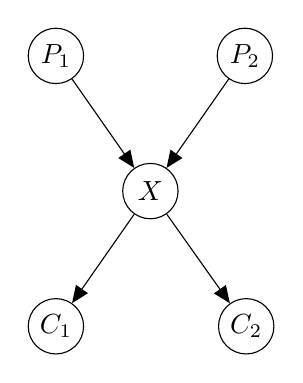
\begin{tikzpicture}

  % Define nodes
  \node[latent]                               (c1) {$C_1$};
  \node[latent, right= 1.7 cm of c1]            (c2) {$C_2$};
  \node[latent, above=of c1, xshift= 1.2 cm] (y)  {$X$};
  \node[latent, above=of y, xshift=-1.2cm] (p1) {$P_1$};
  \node[latent, above=of y, xshift=1.2cm]  (p2) {$P_2$};

  % Connect the nodes
  \edge {p1,p2} {y} ; %
  \edge {y} {c2} ;
  \edge {y}{c1};

  % Plates
  %\plate {} {(p1)(p2)(p3)(y)} {$Factor_1$} ;
  %\plate {yx} {(y)(s11)(s12)(c2)} {$Factor_2$};
  %\plate {} {(y)(s2)(c1)(yx.north west)(yx.south west)} {$Factor_3$} ;
  %\plate {} {(w)(y)(yx.north west)(yx.south west)} {$M$} ;

\end{tikzpicture}
%\endpgfgraphicnamed

%%% Local Variables: 
%%% mode: tex-pdf
%%% TeX-master: "example"
%%% End: 

      \end{tabular}
     \hspace{5em}
      \begin{tabular}{cc}
      % model_pca.tex
%
% Copyright (C) 2012 Jaakko Luttinen
%
% This file may be distributed and/or modified
%
% 1. under the LaTeX Project Public License and/or
% 2. under the GNU General Public License.
%
% See the files LICENSE_LPPL and LICENSE_GPL for more details.

% PCA model

%\beginpgfgraphicnamed{model-pca}
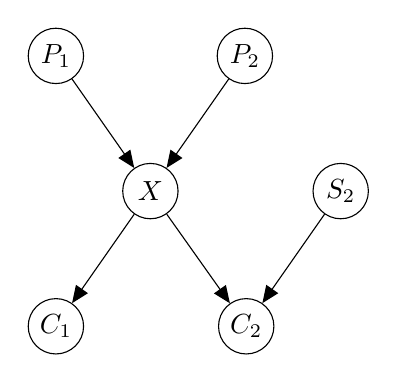
\begin{tikzpicture}

  % Define nodes
  \node[latent]                               (c1) {$C_1$};
  \node[latent, right= 1.7 cm of c1]            (c2) {$C_2$};
  \node[latent, above=of c1, xshift= 1.2 cm] (y)  {$X$};
  \node[latent, above=of c2, xshift= 1.2 cm] (s)  {$S_2$};
  \node[latent, above=of y, xshift=-1.2cm] (p1) {$P_1$};
  \node[latent, above=of y, xshift=1.2cm]  (p2) {$P_2$};

  % Connect the nodes
  \edge {p1,p2} {y} ; %
  \edge {y} {c2} ;
  \edge {y}{c1};
  \edge {s}{c2};

  % Plates
  %\plate {} {(p1)(p2)(p3)(y)} {$Factor_1$} ;
  %\plate {yx} {(y)(s11)(s12)(c2)} {$Factor_2$};
  %\plate {} {(y)(s2)(c1)(yx.north west)(yx.south west)} {$Factor_3$} ;
  %\plate {} {(w)(y)(yx.north west)(yx.south west)} {$M$} ;

\end{tikzpicture}
%\endpgfgraphicnamed

%%% Local Variables: 
%%% mode: tex-pdf
%%% TeX-master: "example"
%%% End: 

    \end{tabular}
  \caption{Two example networks}
\end{figure}

%%%%%%%%%%%%%%%%%%%%%%%%%%%%%%%%%%%%%%%%%%%%%%%%%%%%%%%%%%%%%%%%%%%%%%%%%%%%%%%%%%%%%%

\section{Extension to Multiple Continuous Variables}
\label{sec:multi_var}

\subsection{Discretization of Multiple Continuous Variables}

If there are multiple continuous variables in a Bayesian network, we iterate the one-variable discretization method discussed above for all continuous variables. While discretizing a continuous variable, other continuous variables must be discretized, either by a prediscretization that was done before the first iteration or by the discretization result of the latest iteration. The prediscretization can be done by equal-width discretization, which is defined as follows:
\begin{equation}
M_X =  \{ min_X, min_X + \delta, min_X + 2\delta, \ldots, \delta, max_X \},
\end{equation}
where $min_X$ and $max_X$ are minimal and maximal values of $D_X$, respectively, $\delta =  (max_X - min_X)/k$, and $k$ is the desired number of intervals after equal-width discretization. $k$ is same for all continuous variables and is set to be median value of all discrete variables' cardinalities. After prediscretization, we iterate the one-variable discretization on each continuous variable in the following order: from the continuous variable with highest topological order (leaves) to the continuous variable with lowest topological order (root). We call one such series of discretizations as a cycle. The advange of the order is that, for the first cycle of iteration, we can use less number of unsupervised discretization result. For example, in the right graph of Figure 2, assume $S_2$ is the only discrete variable. If we begin the iteration with $P_1$, then the discretization of $P_1$ will involve the prediscretization results of both $P_2$ and $X$. However, if we begin the iteration with $C_1$, then the discretization of $C_1$ will only involve the prediscretization result of $X$.

When the number of intervals after discretization and the positions of discretization edges converge, we stop the iterations and output the discretization policy on each continuous variable. Since the convergence is not guaranteed, we also set up a maximal number of cycles to prevent infinite iterations. In our test on real-world data, the iteration results usually converge within few cycles. Even if it does not converge, 10 cycles usually produce good enough discretization result. The pseudocode of multi-variable discretization is shown in Algorithm 2, where we require four inputs: $D''$, the mixed data of all variables that we plan to learn from, $G$, the network structure, $C$, the set of all continuous variables in a reverse topological order, and $u_{cycle}$, the upper bound of times of cycles.

\begin{algorithm}
\caption{ Discretization of multiple continuous variables}
\begin{algorithmic}[5]
\Function{Discretize}{$D''$, $G$, $C$, $u_{cycle}$}
\State
\State $M[i] \leftarrow$ the discretization policy of $i$th variable
\State $n \leftarrow$ the number of variables in Bayesian network
\State $D^*_i \leftarrow M[i] (D_i)$, the discretized $D_i$ by $M[i]$
\State $D^* \leftarrow $ the discretized data for all variables, where $D^*_i \leftarrow D''_i$ if $i \notin C$
\State $k \leftarrow median\{ \|v\|, v\notin C\}$
\State
\For {$i = 1$ to $n$}
\If {$i \in C$}
\State $M[i] \leftarrow$  equal-width discretization with $k$ intervals
\State $D^*_i \leftarrow  M[i] (D''_i)$
\EndIf
\EndFor
\State
\State $cycle \leftarrow 0$
\While {$M$ is not converged  \textbf{and} $cycle \leq u_{cycle}$}
\State {$cycle  \leftarrow cycle  + 1$}
\For {$j = 1$ to $\|C\|$}
\State $D^*_{\backslash C(j)} \leftarrow D^*$ without $D^*_{C(j)}$.
\State {$M[C(j)] \leftarrow $ DISCRETIZE($D_{C(j)}$,$D^*_{ \backslash C(j)}$,graph)}
\State {$D^*_{C(j)}  \leftarrow$ $M[C(j)](D''_{C(j)}) $}
\EndFor
\EndWhile
\State \Return $M$
\EndFunction
\end{algorithmic}
\end{algorithm}

\subsection{Discretization of Continuous Variables While Structure Learning}

In many situations the network structure is not known in advance, then we need to learn it from data. We use an alternative approach to combine our proposed discretization method with the K2 structure learning algorithm \citep{K2}. That is to say, we start with some prediscretizations on continuous variables and run the K2 algorithm given the discretized data. Each time an edge is added by the K2 algorithm, we rediscretize the continuous variables based on the current network. Then the new discretization policies update the discretized data of all continuous variables, and we continue the next K2 step with the updated discretized data. This cycle is repeated until no edge is added by the K2 algorithm. The detail of the procedure is shown in Algorithm 3. Here we have five inputs: $D'$, the mixed data we plan to learn from, $C$, the set of all continuous variables, $order$, the variable order which is required by the $K2$, $u_{parent}$, the upper bound of number of parents which is also required by the $K2$, and $u_{cycle}$, the upper bound of times of cycles. Notice that in the usual structure learning from discrete data, one usually run the K2 algorithm many times with different orders, and choose the structure with the highest K2 score. We do the same thing: run Algorithm 3 many times, each time with a different order, and pick the discretized Bayesian network with the highest K2 score.
\begin{algorithm}
\caption{ Learning a discrete-valued Bayesian network}
\begin{algorithmic}[5]
\Function{Learn\_DBN}{$D''$, $C$, $order$, $u_{parent}$, $C$, $u_{cycle}$}
\State

\State $n \leftarrow$ the number of variables in Bayesian network
\State $k \leftarrow median\{ \|v\|, v\notin C\}$
\State $M[i] \leftarrow$ the discretization policy of $i$th variable
\State $D^*_i \leftarrow M[i] (D_i)$, the discretized $D_i$ by $M[i]$
\State $D^* \leftarrow $ the discretized data for all variables, where $D^*_i \leftarrow D''_i$ if $i \notin C$
\State $G \leftarrow$ the initial graph (no edges between nodes)
\State
\For {$i = 1$ to $n$}
\If {$i \in C$}
\State $M[i] \leftarrow$  equal-width discretization with $k$ intervals
\State $D^*_i \leftarrow  M[i] (D''_i)$
\EndIf
\EndFor
\State
\For {$i =1$ to $n$}
\State $P_{old} \leftarrow f(X^*_i,\Pi_{X^*_i})$: Equation 5
\State OKToProceed $\leftarrow$ \textbf{true}
\While OKToProceed \textbf{and} $\|\Pi_{X^*_i}\| < u_{parent}$
\State $Y \leftarrow$ an element from the set $order[1:i] \backslash \Pi_X$
\State $P_{new} \leftarrow f(X^*_i,\Pi_{X^*_i} \cup Y)$
\If {$P_{new} > P_{old}$}
\State $P_{old} \leftarrow P_{new}$
\State $\Pi_{X_i} \leftarrow \Pi_{X_i} \cup Y $
\State $M \leftarrow$ {DISCRETIZE}({$D''$, $G$, $C$, $u_{cycle}$}): Algorithm 2
\State $D* = M(D'')$
\Else
\State OKToProceed $\leftarrow$ \textbf{false}
\EndIf
\EndWhile
\EndFor
\State \Return $G$, $M$
\EndFunction
\end{algorithmic}
\end{algorithm}

%%%%%%%%%%%%%%%%%%%%%%%%%%%%%%%%%%%%%%%%%%%%%%%%%%%%%%%%%%%%%%%%%%%%%%%%%%%%%%%%%%%%%%

\section{Experiments}
\label{sec:experiments}



%\begin{acknowledgements}
%If you'd like to thank anyone, place your comments here
%and remove the percent signs.
%\end{acknowledgements}

% BibTeX users please use one of
%\bibliographystyle{spbasic}      % basic style, author-year citations
%\bibliographystyle{spmpsci}      % mathematics and physical sciences
%\bibliographystyle{spphys}       % APS-like style for physics
%\bibliography{}   % name your BibTeX data base

% Non-BibTeX users please use
%\begin{thebibliography}{}
\bibliographystyle{spbasic}
\bibliography{my_bib}

%%%%%%%%%%%%%%%%%%%%%%%%%%%%%%%%%%%%%%%%%%%%%%%%%%%%%%%%%%%%%%%%%%%%%%%%%%%%%%%%%%%%%%

\section*{Appendices}

\begin{algorithm}
\caption{ Calculation of function $h(u,v)$ for all $u \leq v$}
\label{alg:h}
\begin{algorithmic}[1]
\State Initialize $H$ as an $N \times N$ matrix that all elements are 0.
\State $count_p$ is an $N \times N \times \|\Pi_X\|$ matrix such that $count_p [u,v,w]$ is the number of instances from $x_u$ to $x_v$ with $w$th value of $\Pi_X$. This matrix can be calculated in $O(\|\Pi_X\| \cdot N^2)$
\For {$u = 1$ to $N$}
\For {$v = u$ to $N$}
\State $H(u,v) \leftarrow H(u,v) + \log((v-u + J_p)!) - \log((J_p -1)!)$
\For {$w = 1$ to $\|\Pi_X\|$}
\State $H(u,v) \leftarrow H(u,v) - \log( count_p(u,v,w)!)$
\EndFor
\EndFor
\EndFor

\For {$j = 1$ to $n_c$}
\State XXX
\EndFor
\end{algorithmic}
\end{algorithm}

\end{document}
% end of file template.tex

